\subsection{Architecture}
Autoformer (\citet{https://doi.org/10.48550/arxiv.2106.13008}) makes substantial modifications to the building blocks of Transformer. 
As shown in Figure \ref{fig:autoformer}, the multihead attention module is replaced by the autocorrelation module, and layer normalization module by decomposition module. 
The idea is to emulate the traditional seasonal-trend decomposition (\citet{cleveland90}) while leverage the flexibility of neural networks to model periodic patterns. 

\begin{figure}
    \centering
    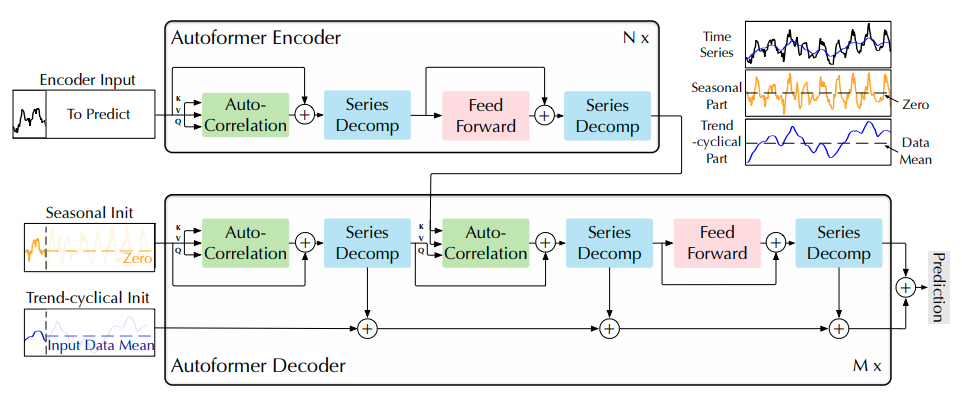
\includegraphics[width=0.8\textwidth]{img/autoformer.png}
    \caption{A visualization of Autoformer architecture.}
    \label{fig:autoformer}
\end{figure}

\subsubsection{Decomposition Module}
The module aims at decomposing the input signal $X \in \Rb^L$ into trend $T \in \Rb^L$ and seasonality $S \in \Rb^L$ such that $X = T + S$. 
The trend is expected to contain long-term non-stationary changes, whereas seasonality is more concerned about cyclical patterns. 
To this end, we just compute moving average (i.e. perform average pooling) along the temporal domain to obtain the trend, and substact it element-wise to get seasonality. 
Mathematically, we have \begin{align*}
    T &= \text{AvgPool}(X) & S &= X - T.
\end{align*}

Notice in Figure \ref{fig:autoformer} that the input into the decoder gets decomposed in the beginning, which, we hypothesize, gives an appropriate \textit{baseline} for later forecasting. 
As noted by \citet{https://doi.org/10.48550/arxiv.2202.07125}, the decomposition mechanism indeed boosts all Transformer variants' performance significantly. 
These ideas will be revisited in our experiments. 

\subsubsection{Autocorrelation Module}
This module emulates the idea of autocorrelation to compute sequence-level similarities in hope of capturing period-based dependencies. 
More formally, the similarity between a query sequence $Q \in \Rb^{L}$ and a $\tau$-delayed key sequence $K \in \Rb^{L}$ is defined as $$R_{Q, K}(\tau) = \sum_{t = 1}^L Q_tK_{t - \tau}.$$
The intuition is that $R_{Q, K}(\tau)$ will be large in magnitude if two sequences are similar and have period $\tau$. 
To optimize memory and speed consumptions, only top-$k$ different $\tau$'s that give high $R_{Q, K}(\tau)$ are selected and normalized by \texttt{softmax} to be attention weights $\{\alpha_{\tau_i}\}_{i = 1}^k$. 
Finally, the output is the linear combination of $k$ different wrap-arounded (i.e. \texttt{Roll}-ed) value sequences $V \in \Rb^{L}$: $\sum_{i = 1}^k \alpha_{\tau_i} \text{Roll}(V, \tau_i)$ (see Figure \ref{fig:autocorrelation}). 

\begin{figure}
    \centering
    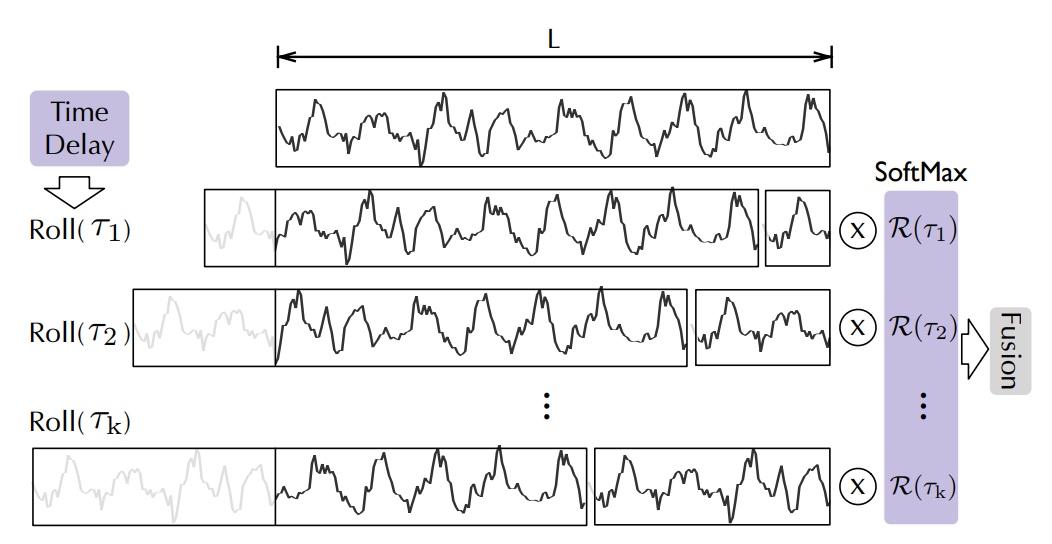
\includegraphics[width=0.6\textwidth]{img/autocorrelation.png}
    \caption{A visualization of autocorrelation module.}
    \label{fig:autocorrelation}
\end{figure}

For efficient computation of $R_{Q, K}(\tau)$, the model employs the Fast Fourier Transforms. 
We refer the interested readers to the original paper for more details. 

\subsection{Experiments}
The experiments are designed to explain the superior performance brought about by the decomposition module and autocorrelation module, respectively, and investigate their robustness under different regularities. 
On top of real-world benchmarks, we generate nine synthetic datasets of various characteristics. 
Except stated explicitly, the models are trained and evaluated under the same hyperparameter setting. 

\subsubsection{Datasets}
To avoid complicating the analysis, all synthetic datasets are univariate ($d = 1$) with the same length, that is, 8k timestamps. 
We take one untrended dataset, \texttt{sinx}, as an example to illustrate the data generation process. 
To begin, we initialize a equally spaced sequence of length 8k: $$X = [\cdots, -0.75, -0.50, -0.25, 0., 0.25, 0.50, 0.75, \cdots].$$
Then, we feed it into some pre-defined function (\texttt{sin} in this case). 
Finally, Gaussian noise with zero mean and appropriate standard deviation is added. 
Importantly, we make the underlying period (if any) so small that the length of the encoder input (see Figure \ref{fig:sinx}) is sufficient to discover periodicity. 

\begin{figure}
    \centering
    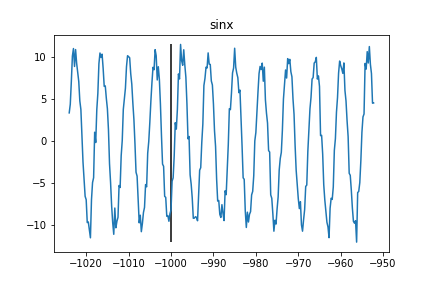
\includegraphics[width=0.5\textwidth]{img/data_sinx.png}
    \caption{A subsequence of the entire \texttt{sinx} dataset. 
    To the left of the black vertical line is fed into the encoder, while to the right is to be predicted. 
    The encoder \textit{should} be able to discover the periodicity.}
    \label{fig:sinx}
\end{figure}

Our synthetic datasets can be categorized into trended (i.e. containing underlying trend) and untrended (i.e. oscilating around 0). 
As for the oscilation, one underlying cycle corresponds to approximately 25 timestamps or length of 6 on the real line. 
Denoting standard Gaussian noise by $\Nc$, we present an overview of different datasets as follows. 
Readers may proceed to Appendix \ref{app:data} for visualizations of all datasets. \begin{itemize}
    \item Trended \begin{itemize}
        \item \texttt{x}: $Y = X + \Nc$. This is just a canonical trend. 
        \item \texttt{sinx\_x}: $Y = 10\sin X + X + \Nc$. It additively combines the canonical trend with a cyclical pattern. Signal-trend decomposition should work well in this case. 
        \item \texttt{sinx\_sqrtx}: $Y = 10\sin X + 20\sqrt{X - \min(X)} + \Nc$. The trend is non-linear and, more specifically, concave downward. 
        \item \texttt{sinx\_x2\_sym}: $Y = 10\sin X + (\frac{X}{50})^2 + \Nc$. The trend is symmetric and concave upward. 
        \item \texttt{sinx\_x2\_asym}: $Y = 10\sin X + (\frac{X - \min(X)}{30})^2 + \Nc$. The trend is assymetric and concave upward. The training and test datasets have drastically different means. 
    \end{itemize}
    \item Untrended \begin{itemize}
        \item \texttt{sinx}: $Y = 10\sin X + \Nc$. This is just a canonical periodic pattern. Autocorrelation module should be able to capture it. 
        \item \texttt{xsinx}: $Y = e^{X \mod 4} \dot (10\sin X + \Nc)$. The amplitude varies over time. 
        \item \texttt{sinx\_sin2x\_sin4x}: $Y = 10\sin X + 10\sin 2X + 10\sin 4X + \Nc$. The periodic pattern is more complicated. 
        \item \texttt{sinx\_c}: $Y = 10\sin X + (-1)^{\mathbb{I}[X \mod 16 < 8]} 30 + \Nc$. Each subsequence is shifted either upward or downward, requiring greater flexibility to capture these drastic changes. 
    \end{itemize}
\end{itemize}

Meanwhile, we also perform ablation studies on the aforementioned real-world datasets. Detailed dataset descriptions can be found in Section \ref{benchmarks}. 

\subsubsection{Results}

According to Figure \ref{fig:trended_mse}, when there is an underlying trend, incorporating decomposition module improves the model performance significantly. 
Instead, if we naively employ autocorrelation module without a proper detrending process, the model can get even more confused. 
On the other hand, if there is no trend in the first place, decomposition module can in fact create negative impacts, possibly by introducing random noise. 

\begin{figure}
    \centering
    \begin{subfigure}{0.6\textwidth}
        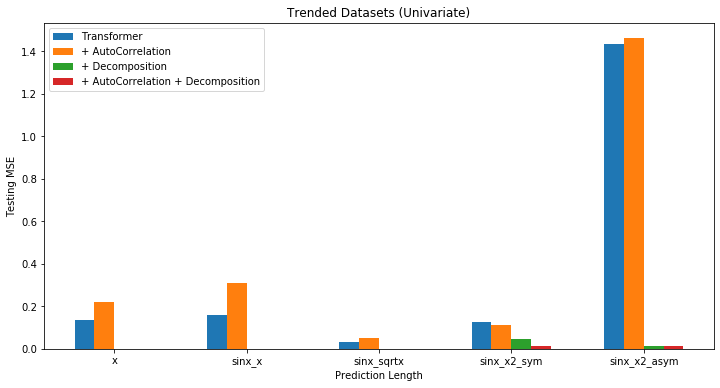
\includegraphics[width=\textwidth]{img/mse_trended.png}
    \end{subfigure}
    \begin{subfigure}{0.6\textwidth}
        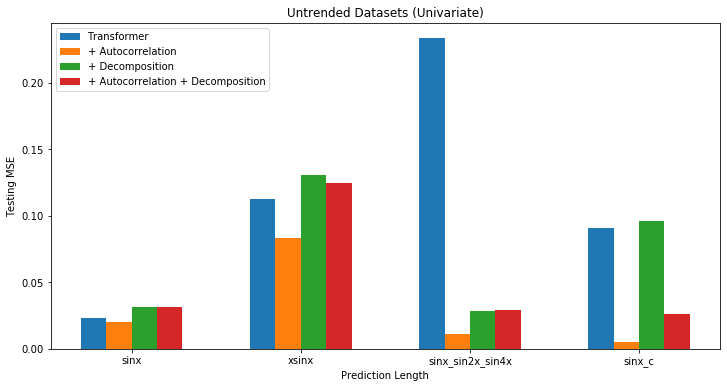
\includegraphics[width=\textwidth]{img/mse_untrended.png}
    \end{subfigure}
    \caption{Mean square errors on trended and untrended synthetic datasets. The \texttt{+ AutoCorrelation + Decomposition} case is equivalent to the Autoformer.}
    \label{fig:trended_mse}
\end{figure}

Figure \ref{fig:synth_pred} plots the forecasting results of a randomly chosen subsequence. 
Plots for other datasets can be found in Appendix \ref{app:pred}. 
As expected, the decomposition module \textit{recalibrate} the prediction baseline to an appropriate level, so the final results would not deviate too much from the target. 

\begin{figure}
    \centering
    \begin{subfigure}{0.9\textwidth}
        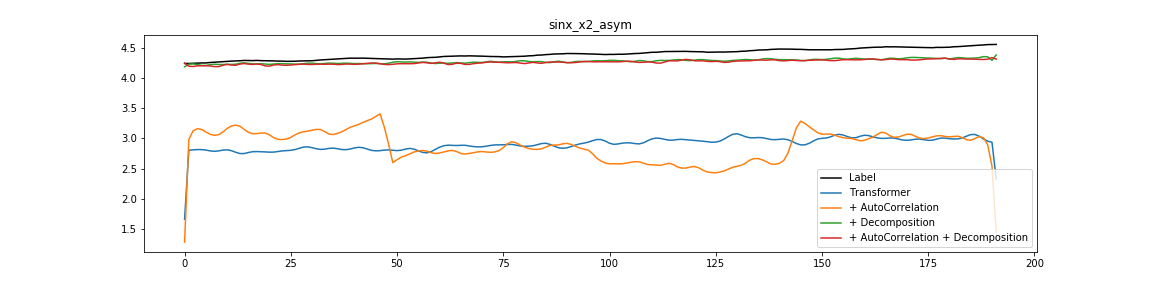
\includegraphics[width=\textwidth]{img/pred_sinx_x2_asym.png}
    \end{subfigure}
    \begin{subfigure}{0.9\textwidth}
        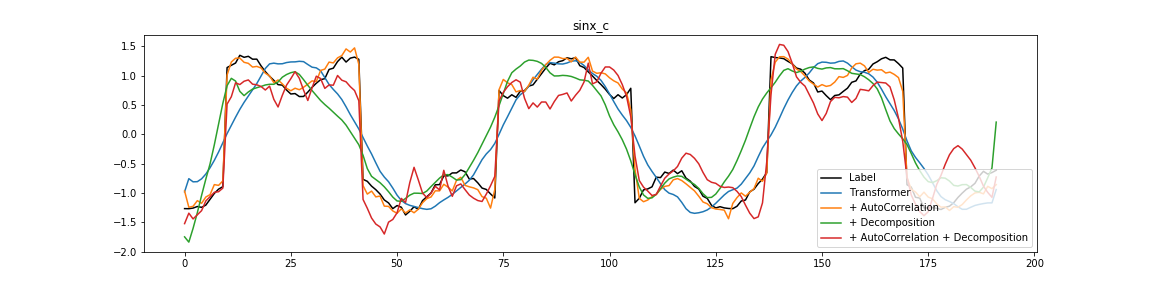
\includegraphics[width=\textwidth]{img/pred_sinx_c.png}
    \end{subfigure}
    \caption{Forecasting plots of a random subsequence in one trended and one untrended synthetic datasets.}
    \label{fig:synth_pred}
\end{figure}

Since decomposition module simply computes the running average, the size of sliding window is a hyperparameter. 
Recall that by construction, one period corresponds to approximately 25 timestamps. 
Thus, we may expect models with sliding window size an integer multiple of 25 to achieve better performance. 
Figure \ref{fig:lwin} indeed confirms our expectation and emphasizes the importance of choosing an appropriate window size. 

As for the autocorrelation module, we notice that as long as the signal has been detrended, it is capable of improving the forecasting quality. 
This phenomenon is especially pronounced when we know beforehand that the data is untrended, so no decopmosition is performed to avoid introducing noise. 

\begin{figure}
    \centering
    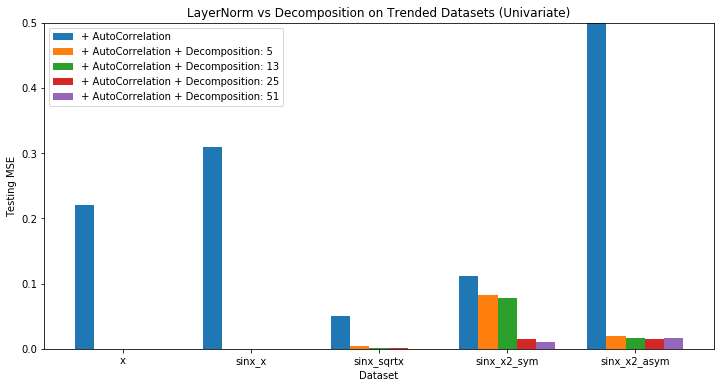
\includegraphics[width=0.6\textwidth]{img/mse_trended_decomp.png}
    \caption{Mean square errors of models with varying decomposition window sizes.}
    \label{fig:lwin}
\end{figure}

Furthermore, we can explore the explainability of autocorrelation weights, just like the attention weights. 
We expect that the top-$k$ most significant $\tau$'s will include an integer multiple of 25 very often. 
Unfortunately, Figure \ref{fig:tau_synth} shows a case where the distribution of $\tau$ does not align with our intuition. 
More examples can be found in Appendix \ref{app:tau}. 
Most of the time, the distribution of $\tau$ does not seem to offer insight into the underlying periodicity of the data. 
Therefore, the working mechanism of the autocorrelation module appears to be a black box awaiting for future discovery. 

\begin{figure}
    \centering
    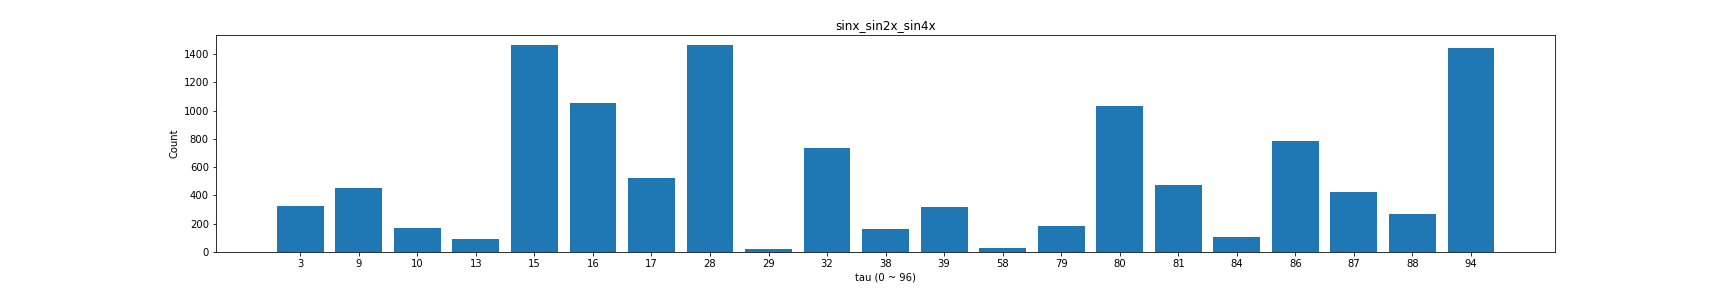
\includegraphics[width=\textwidth]{img/tau_sinx_sin2x_sin4x.png}
    \caption{For each $\tau$, the number of times $R_{Q, K}(\tau)$ is a top-$k$ largest one.}
    \label{fig:tau_synth}
\end{figure}

\begin{figure}
    \centering
    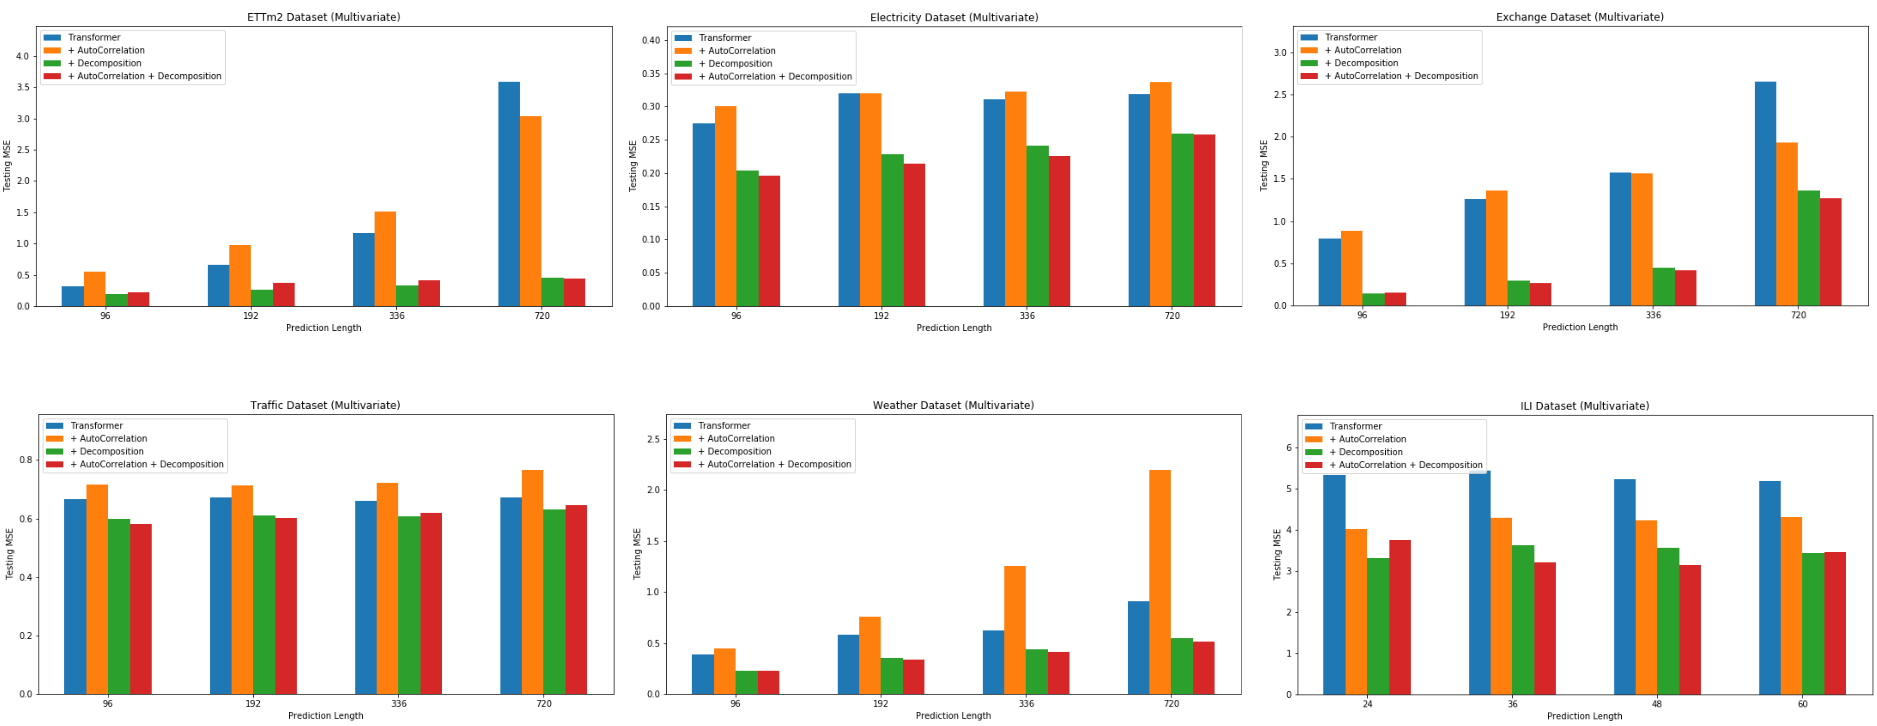
\includegraphics[width=\textwidth]{img/mse_real.png}
    \caption{Mean square errors vanilla Transformer and its variants on real-world datasets.}
    \label{fig:mse_real}
\end{figure}

Finally, we show the results on real-world datasets in Figure \ref{fig:mse_real}. 
The baseline model is vanilla Transformer and we replaces the attention module by autocorrelation module and/or layer normlization module by decomposition module. 
Consistent with findings due to \citet{https://doi.org/10.48550/arxiv.2106.13008}, the greatest empirical improvement comes from the decomposition module. 
However, the effect of autocorrelation module is more nuanced. 
This is possibly because the trend is harder to be identified and removed, and the underlying cyclical patterns are more complicated. 
While harder to interpret, the prediciton plots is also available in Appendix \ref{app:pred}. 
